\chapter{Results and Discussion}  \label{Ch:4}

\section{Development Results}
The methodology of construction of the novel force sensor as detailed in section \ref{sec:forcesens}, the novel force-sensor was built using the speechifications listed in the section to produce a physical version used for the comparison experiment shown in Figure: \ref{fig:loadcelltest}.\\
The novel force sensor array has been found to be able to measure the correct amount of force applied to each of the load cells in the applied direction.


\section{Results from the Experiment on force sensor}
from the experiment performed in section \ref{sec:experiment}, the force magnitude from each load cell collected from the python code \ref{code:py}, are then plotted in MATLAB, showing the significance of applying a force on the other load cells.\\
the first experiment carried out was to apply force only in the vertical axis and measure co-linearities measures across the other load cells, the results from this experiment are shown in Figure:\ref{fig:matlab1}, and from the plot we can see from 1 to 300, the forces applied is only read majorly by the y-axis load cell but after that, there is a lot of interference in the other load cells, mostly due to the unstable structure will allows the load cells to move and couple each other.\\
For the second experiment, varied force is applied in the positive and negative directions of each axis to see the effect, shown in Figure \ref{fig:matlab2}. It is seen that when negative and positive y forces are applied there is little effect on the other load cells, unlike the z-axis where negative z shows a very large deflection on the other load cells, same for the x-axis load cell as well.

\begin{figure}[p]%matlab result graph 1
	\centering
	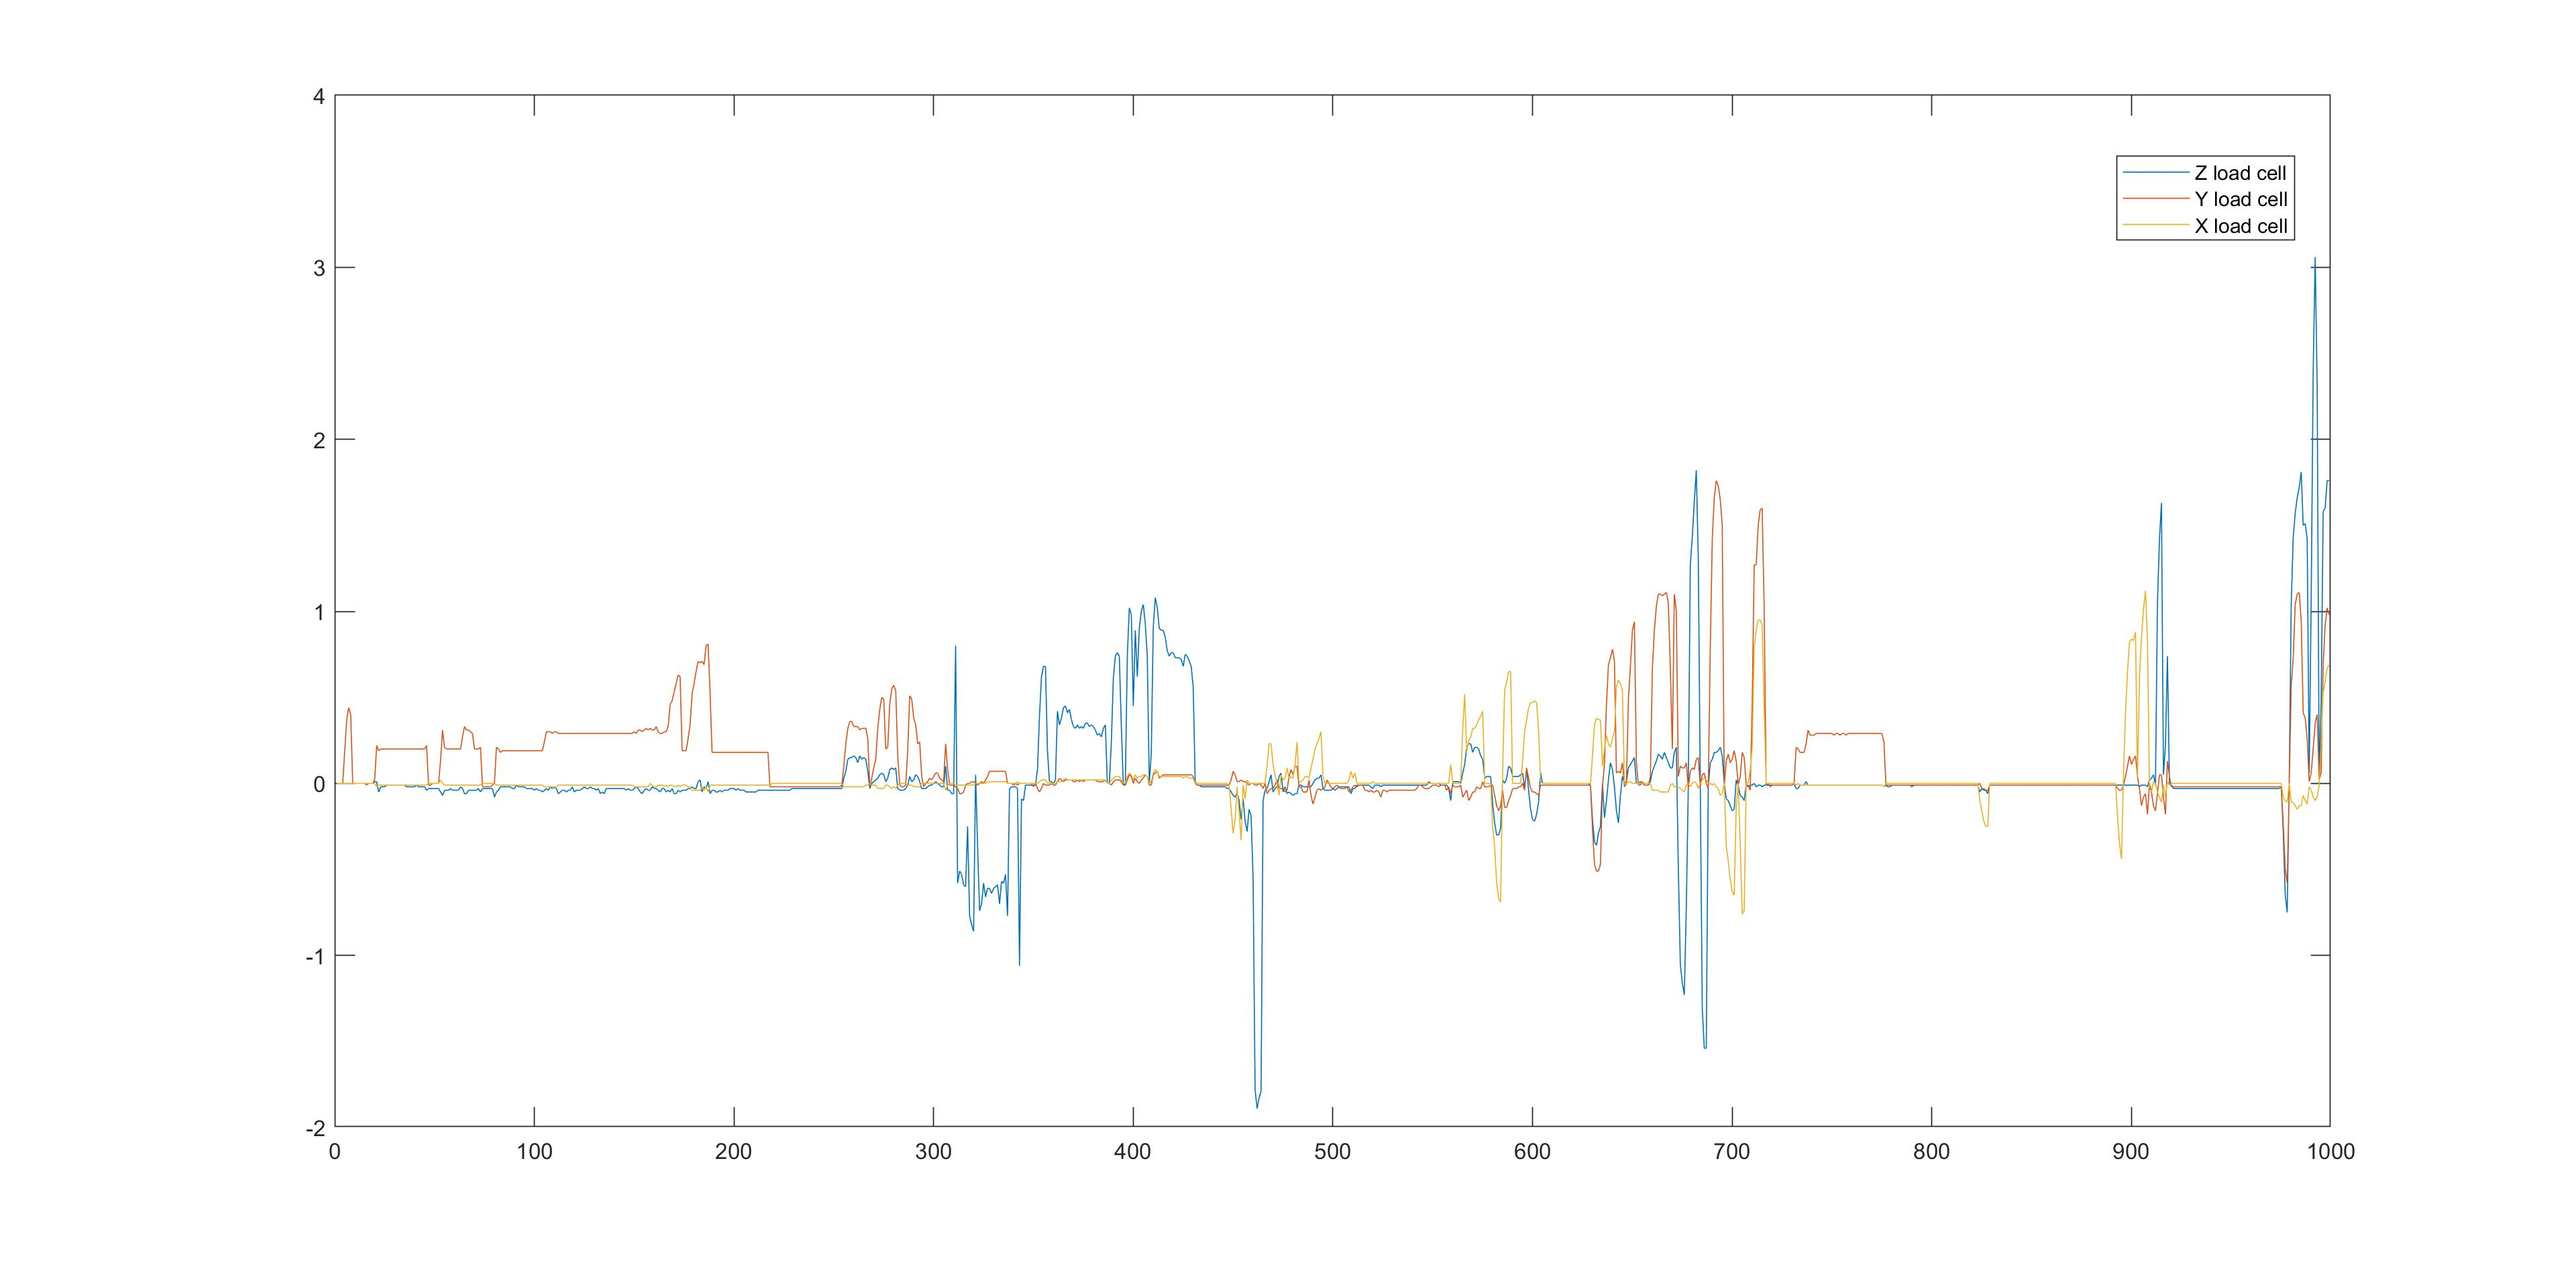
\includegraphics[width=1.2\linewidth]{figures/ch4/matlabresult1}
	\caption{Figure showing one of the test}
	\label{fig:matlab1}
\end{figure}


\begin{figure}[p]%matlab result graph2
	\centering
	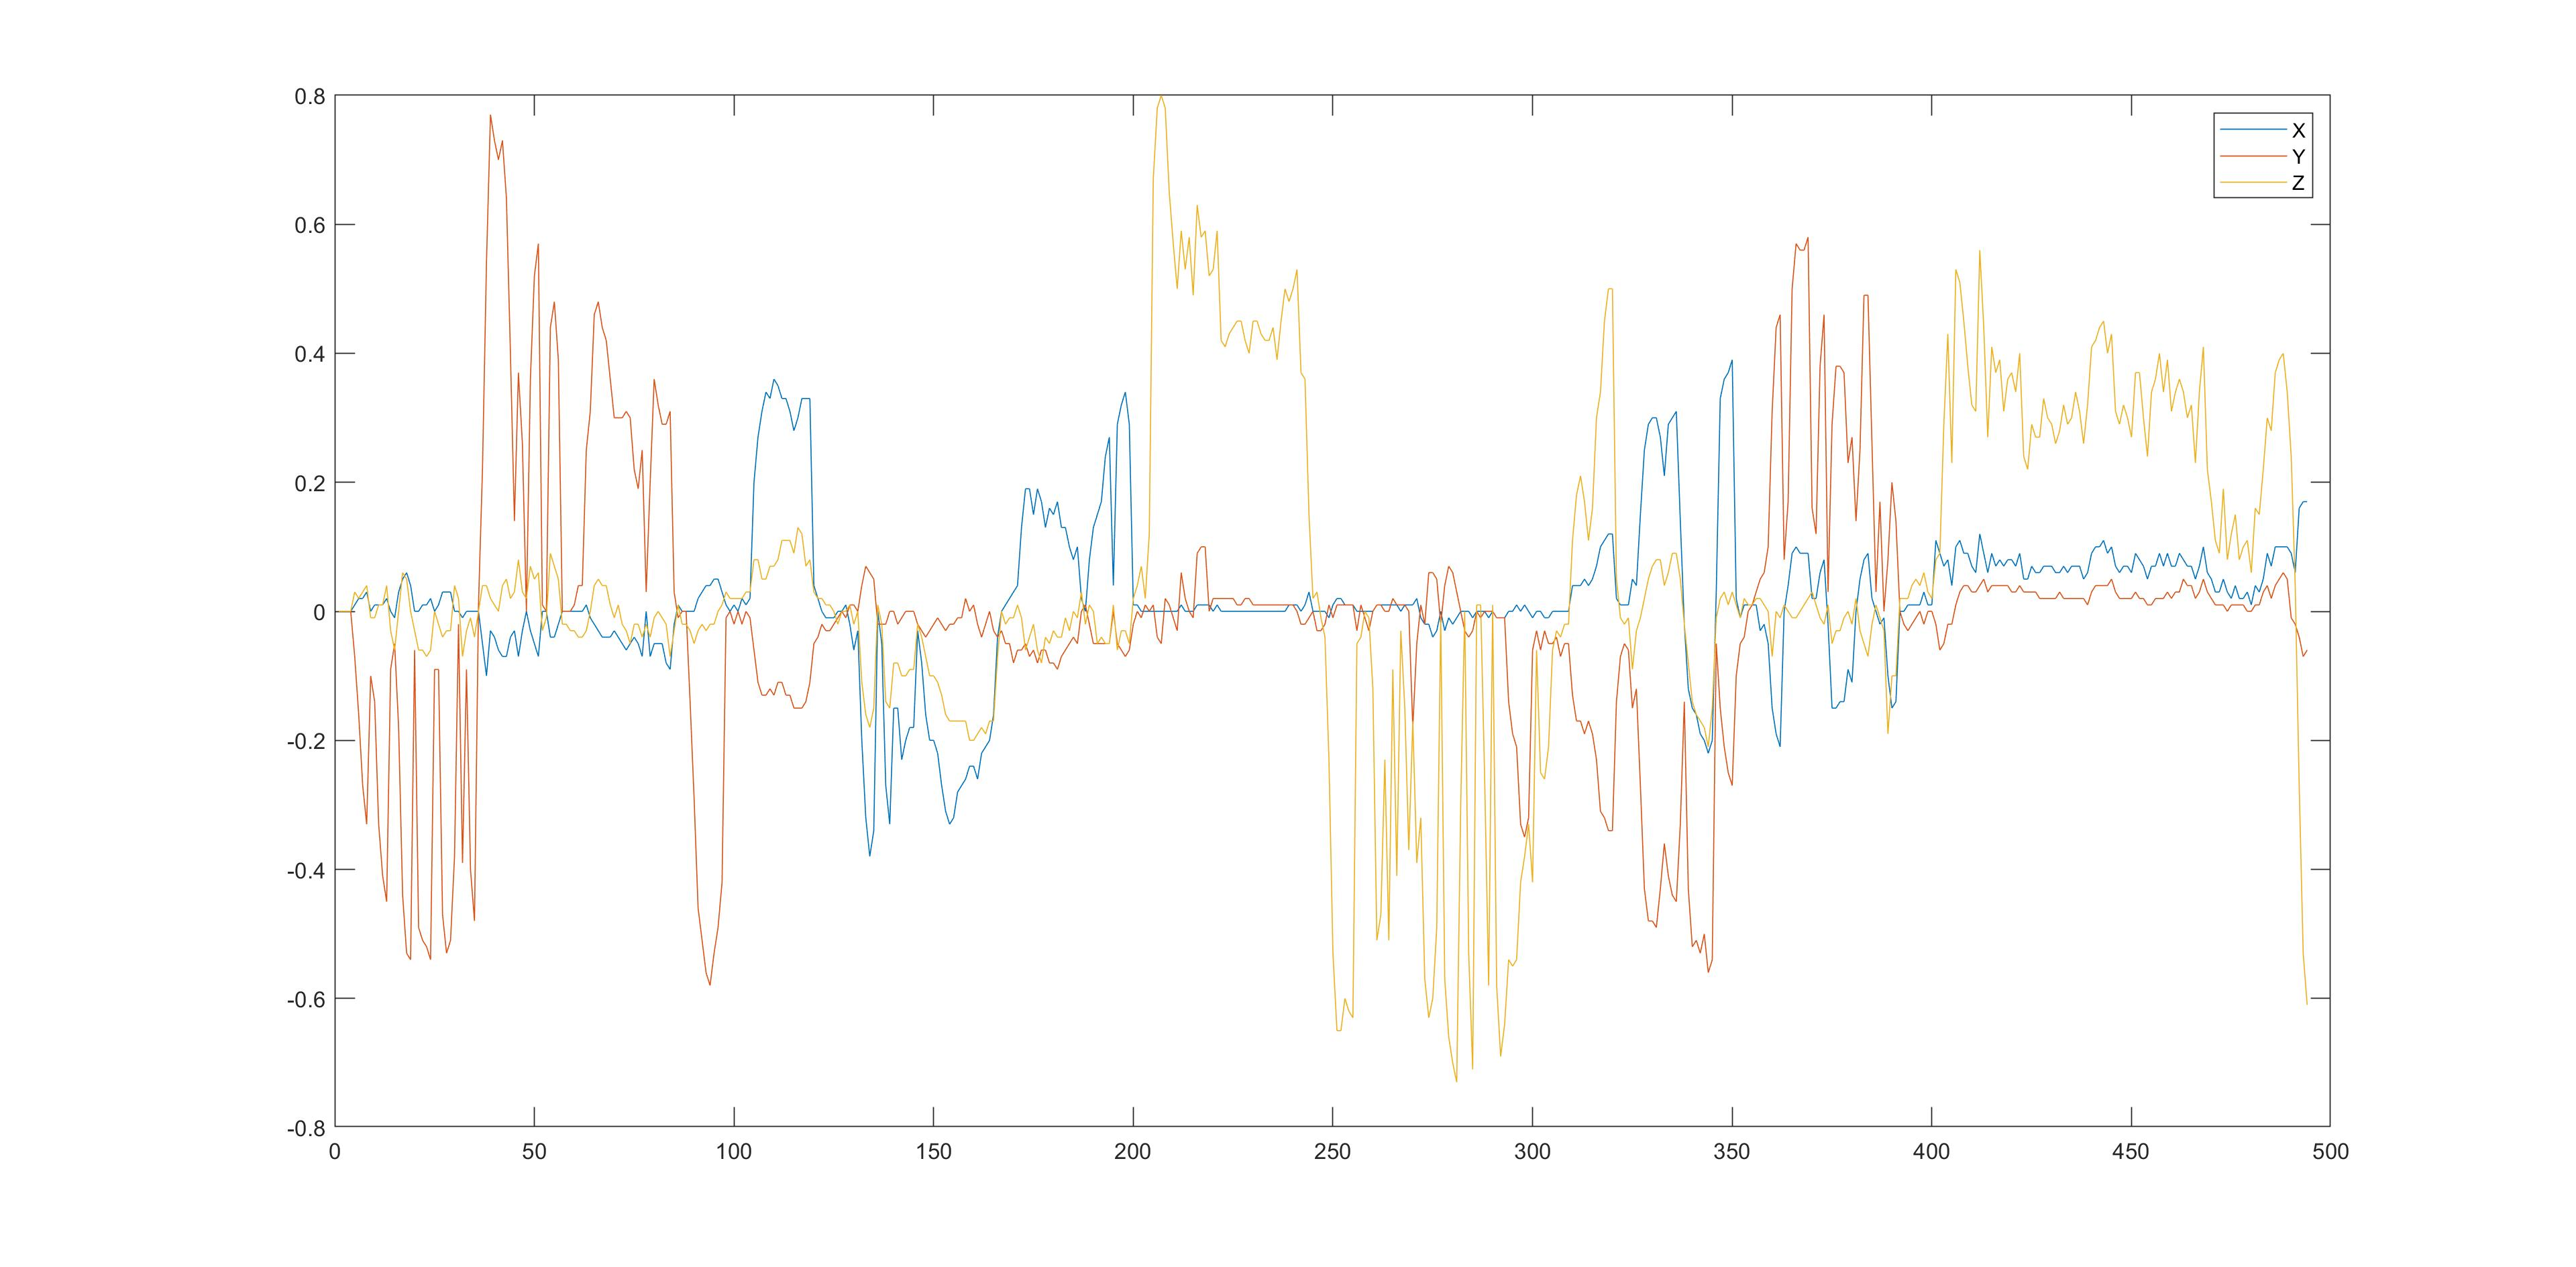
\includegraphics[width=1.2\linewidth]{figures/ch4/matlabresult2}
	\caption{Figure showing another test}
	\label{fig:matlab2}
\end{figure}

\section{Result of the \ac{blue} demonstration version}
The development version of \ac{blue} has been completed and is able to visually show a bilateral robot and a implementation of a hybrid control scheme combining a active assist and the master slave control scheme.\\
making use of the design: \ref{fig:bluepres}, and the code: \ref{code:arduinomaster} in combination with a python gui code and physical structure is completed and able to be used.

\section{Conclusion of Transfer Learning approach}
Transfer learning is a broad area with multiple methods that can be implemented to solve a problem that requires the use of transfer learning.\\
the first choice to use was the inductive transfer, followed by transductive, both methods failed to be suitable for implementation due to the fact that they are methods only for classification tasks. Since the problem in question to be solved, i.e. the prediction of values from a force sensor is a regression problem, this requires a regression transfer learning method, and the best method that can be used is found to be a transductive inference method which uses the transductive method but for a regression problem.\\
Therefore the best method for solving the problem of transferring knowledge to reduce calibration times of a force sensor array is the transductive inference.
\section{Discussion}
\subsection{Discussion of Force-sensor results}
From the small data collected from the novel force-sensor shown in Figures \ref{fig:matlab1} and \ref{fig:matlab2}. it can be seen that the novel force sensor system is a usable multi-axis sensor with a lot of co-linearities which can be reduced with machine learning methods such as transfer learning methods in the future.